%\title{emnlp 2017 instructions}
% File emnlp2017.tex
%

\documentclass[11pt,letterpaper]{article}
\usepackage{emnlp2017}
\usepackage{times}
\usepackage{latexsym}
\usepackage{graphicx}
\usepackage{amssymb}
\usepackage{amsmath}

% Uncomment this line for the final submission:
% \emnlpfinalcopy

%  Enter the EMNLP Paper ID here:
\def\emnlppaperid{***}

% To expand the titlebox for more authors, uncomment
% below and set accordingly.
% \addtolength\titlebox{.5in}    

\newcommand\BibTeX{B{\sc ib}\TeX}

\title{Discovering Cognates Using LSTM Networks}

% Author information can be set in various styles:
% For several authors from the same institution:
% \author{Author 1 \and ... \and Author n \\
%         Address line \\ ... \\ Address line}
% if the names do not fit well on one line use
%         Author 1 \\ {\bf Author 2} \\ ... \\ {\bf Author n} \\
% For authors from different institutions:
% \author{Author 1 \\ Address line \\  ... \\ Address line
%         \And  ... \And
%         Author n \\ Address line \\ ... \\ Address line}
% To start a seperate ``row'' of authors use \AND, as in
% \author{Author 1 \\ Address line \\  ... \\ Address line
%         \AND
%         Author 2 \\ Address line \\ ... \\ Address line \And
%         Author 3 \\ Address line \\ ... \\ Address line}
% If the title and author information does not fit in the area allocated,
% place \setlength\titlebox{<new height>} right after
% at the top, where <new height> can be something larger than 2.25in
\author{Shantanu Kumar \and Ashwini Vaidya \and Sumeet Agarwal \\ 
  Indian Institute of Technology Delhi
  \\ {\tt \{ee1130798, ird11278, sumeet\}@iitd.ac.in}}

\date{}

\begin{document}

\maketitle

%%%%%%%%%%%%%%%%%%%%%%%%%%%%%%%%%%%%%%%%%%%%%%%%
\begin{abstract}
In this paper, we present a deep learning model for the task of pairwise cognate prediction. We use a character level model with recurrent architecture and attention that has previously been employed on several NLP tasks. We compare the performance of our model with previous approaches on various language families. We also employ our model specifically to the domain of discovering cognates from Hindi-Marathi to assist the task of lexical resource creation.
\end{abstract}

%%%%%%%%%%%%%%%%%%%%%%%%%%%%%%%%%%%%%%%%%%%%%%%%
\section{Introduction}
Cognates are words across different languages that are known to have originated from the same word in a common ancestral language. For example, the English word `\textit{Night}' and the German `\textit{Nacht}’, both meaning night and English `\textit{Hound}’ and German `\textit{Hund}’, meaning dog are cognates whose origin can be traced back to Proto-Germanic. Traditionally, the identification of cognates was carried out by a historical linguist, using word lists and establishing sound correspondences between words. For some time now, there has been a growing interest in automatic cognate identification techniques. These are useful in determining linguistic distance within a language family, and also to understand the process of language change. 

Most approaches focus on finding similarity measures between a pair of words (e.g. orthographic or phonetic similarity). \citep{hauer2011clustering, inkpen2005similarity,List2016g}. These are used as features for classifiers to identify cognacy for a particular word-pair. Such features are less effective in order to capture generalizations beyond  string similarity. For example, the words \textit{que} in Spanish and \textit{Hvad} in Danish both map to the concept \textsc{WHAT}, but have nothing in common with each other. We would like our model to find generalizations beyond string similarity, in a manner that is closer to the task carried out by a human expert. 

In this paper, we propose an end-to-end recurrent neural network based model \texttt{without} the need for explicit string similarity feature engineering. LSTM (Long Short Term Memory) networks are being used in a extensive range of NLP tasks to build end-to-end systems. LSTMs have been successfully applied to machine translation \citep{bahdanau2014neural}. language modelling \citep{mikolov2010recurrent}, information retrieval \citep{sordoni2015hierarchical} and RTE \citep{snli:emnlp2015}. As LSTM networks are a form of recurrent network (RNN), they fit more naturally to natural language which also has a sequential architecture and follows a linear order, as compared to convolutional networks which are more hierarchical and hence seem natural for images. Even though NLP literature does not support a clear distinction between the domains where CNNs or RNNs perform better, recent works have shown that each provide complementary information for text classification tasks \citep{yin2017comparative}. We do an extensive analysis of our trained models to try to understand the kinds of features it learns to recognize that are important for making the cognate judgements.

While the task of cognate identification is an interesting problem in its own right, it has also been applied to NLP tasks, like sentence alignment in bitexts and improving statistical machine translation models.\cite{Kondrak:2003,Simard:1993:UCA:962367.962411}. Additionally, it has been proposed that cognates can be used to share lexical resources among languages that are closely related \citep{Singh:07b}. This approach may be particularly useful among the languages of South Asia, which are not rich in such resources. Information about cognates can become an important source for assisting the creation and sharing of lexical resources between languages. Therefore, another contribution of this paper is to apply our cognate detection model to a real language pair. We apply the model to the domain of Hindi-Marathi, using a large unlabeled corpus of aligned texts to find cognate pairs.



%%%%%%%%%%%%%%%%%%%%%%%%%%%%%%%%%%%%%%%%%%%%%%%%
\section{Datasets}

The task of cognate identification will make use of word lists taken from the basic vocabulary e.g. kinship terms, body parts, numbers etc. Usually this vocabulary will represent concepts from the language itself and not borrowed items, (although this is also possible at times). Each concept has its equivalent word from a number of language families and cognate information that is provided in the form of cognate class ids.
for different language families contain the cognate class ids for each token, along with its language and concept/meaning label. 

We make use of datasets from three language families: Indo European, the ASJP database \cite{wichmannASJP:2016}, Austronesian \cite{greenhillBlust:08} and Mayan \cite{wichmann:2008}. 


%The data used for the task consists of annotated word lists. The word lists for different language families contain the cognate class ids for each token, along with its language and concept/meaning label. Word pairs are formed using words from the same concept and are assigned a positive cognate label if their cognate class ids match
%We have primarily used the Indo-European language family for our experiments as are target languages (Hindi and Marathi) belong to this family. But we have additionally also test our models on two other families listed below.


For the purposes of this task, we form word pairs using words from the same concept and such a pair is assigned a positive cognate label if its cognate class ids match.


We also use the TDIL Hindi-Marathi sentence-aligned corpus as the large unlabeled data for our final model. This dataset provides a large part of the vocabulary from the both the languages to search for cognates.

%%%%%%%%%%%%%%%%%%%%%%%%%%%%%%%%%%%%%%%%%%%%%%%%
\section{Related Work}
\textbf{Orthographic features based classifier} : \citet{hauer2011clustering} use a number of basic word similarity measures as input to a SVM classifier for cognate prediction. They use features like common bigrams, longest common substring, word length difference etc. The also use features that encode the degree of affinity between pairs of languages.

\textbf{Gap-weighted common subsequences} : \citet{rama2015automatic} uses a string kernel based approach wherein he defines a vector for a word pair using all common subsequences between them and weighting the subsequence by their gaps in the strings. The subsequence based features outperform orthographic word similarity measures.

\textbf{Siamese ConvNet model} : In a recent work, T. Rama introduces CNN based siamese-style model \cite{rama2016siamese} for the task. The model is inspired by image-similarity CNN models. By using deep learning based models, the need for external feature engineering is avoided and the system outperforms previous works for cognate detection.

%%%%%%%%%%%%%%%%%%%%%%%%%%%%%%%%%%%%%%%%%%%%%%%%
\section{Gap-weighted subsequence model}
Before coming to the LSTM based model, we performed a thorough analysis on the performance of the gap-weighted subsequence model.
There were two fundamental drawbacks in using the common-subsequence model (Referred to as \textit{Multiplicative} model). 

Firstly, since the model only looked at common subsequences, it ignored vital information about closely related subsequences such as ’\textit{fa}’ in FATHER and ’\textit{pa}’ in PATER which are cognate words. 
Secondly, this also resulted in very sparse vectors as the feature space size was huge. To overcome these problems, we tried smoothing techniques which resulted in models Hy-Avg, Hy- Norm and Additive.

\subsection{Error Analysis}
\subsection{Modified model}

%%%%%%%%%%%%%%%%%%%%%%%%%%%%%%%%%%%%%%%%%%%%%%%%
\section{Approach}

\begin{figure}[t]
	\centering
	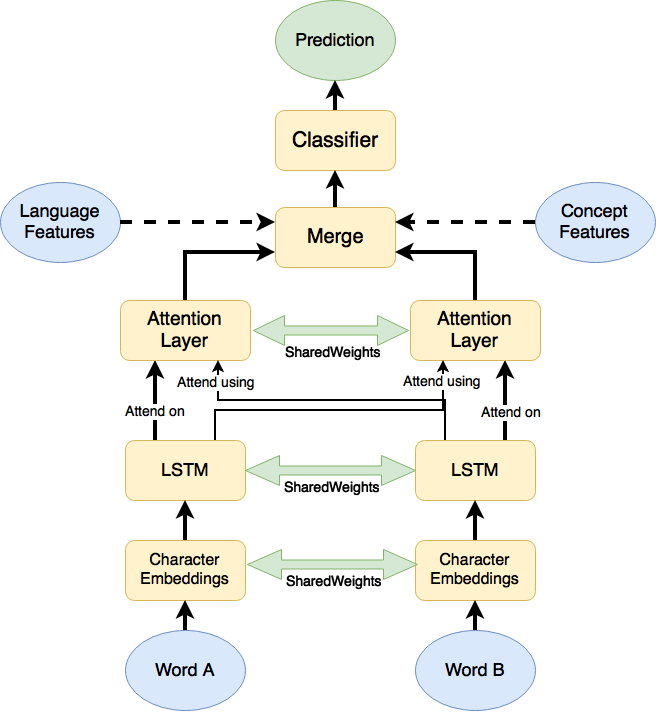
\includegraphics[width=0.35\textwidth]{CoAttNetwork}
    \caption{Recurrent Co-Attention Network for Cognate Discovery}
    \label{CoAttNet}
\end{figure}

The overall model used in our system is called the Recurrent Co-Attention Model (\textit{CoAtt} for short) and is extended from the word-by-word attention model used by \citet{rocktaschel2016reasoning} for the task of recognising textual entailment in natural language sentences. The network used is illustrated in Figure~\ref{CoAttNet}. It is a Siamese style network that encodes a word pair parallely and then makes a discriminative judgement in the final layer. The input words are first encoded into character level embeddings followed by a bidirectional LSTM network and finally a character by character attention layer as described the subsections that follow. The encodings of both the words are merged and passed through a 2-layer neural network with \textit{tanh} and \textit{sigmoid} activations to make a final binary prediction. Additionally we also add a \textit{Language features} vector or a \textit{Concept features} vector to the model by concatenating it with the merged attention vector before passing it to the 2-layer neural network.

%%%%%%%%%%%%%%%%%%%%%%
\subsection{Character Embeddings}

The network starts by encoding the input words into their character embeddings. We encode the words using a character level embedding matrix $E \in \mathbb{R}^{n_e \times |C|}$. Here $n_e$ is the size of the character embeddings and $C$ is the vocabulary of all characters. Thus for an input word $x$ which can be represented as sequence of characters $x = \{c_{i_1}, c_{i_2}, ..., c_{i_n}\}$, is transformed into a sequence of vectors $y = \{e_{i_1}, e_{i_2}, ..., e_{i_n}\}$ where $e_j$ is the $j^{th}$ column of the $E$ matrix. This embedding matrix is learnt during training and each column in the matrix represents the embedding vector of the respective token in the vocabulary. 

\citet{rama2016siamese} manually defined the character embeddings using various properties of the respective phoneme and fixed these embeddings during training. However, we observe that such a method restricts the power of the distributional representation to world knowledge known to us and letting the embeddings be learnt themselves should help learn a representation that is useful for the task in hand.

%%%%%%%%%%%%%%%%%%%%%%
\subsection{LSTM network}

Recurrent Neural networks (RNN) with Long Short-Term Memory (LSTM) have been extensively been used in several NLP tasks. After the input words to the network are encoded using the character embedding matrix, we transform them use LSTM cells. Given the input words $y = \{e_1, e_2, ..., e_n\}$, at every time step $t$ the LSTM of hidden unit size $n_h$ uses the next input $e_t$, the previous output $h_{t-1}$ and the previous cell state $c_{t-1}$ to compute the next output $h_t$ and the next cell state $c_t$ as follows,

\begin{align}
H &= [e_t h_{t-1}] \\
i_t &= \sigma (W^iH + b^i) \\
o_t &= \sigma (W^oH + b^o) \\
f_t &= \sigma (W^fH + b^f) \\
c_t &= i_t * tanh(W^cH + b^c) + f_t * c_{t-1} \\
h_t &= o_t * tanh(c_t)
\end{align}

Here $W^i$, $W^o$, $W^f$, $W^c \in  \mathbb{R}^{n_e+n_h \times n_h}$ and $b_i$, $b_o$, $b_f$, $b_c \in \mathbb{R}^{n_h}$ are trained weights of the LSTM. The final output of the LSTM gives us a sequence $\{h_1, h_2, ..., h_n\}$ for every word, where $h_j \in \mathbb{R}^{n_h}$.

%%%%%%%%%%%%%%%%%%%%%%
\subsection{Attention}

Attention neural networks have been used extensively in tasks like machine translation \cite{}, image captioning \cite{}, summarisation \cite{} and visual question answering \cite{}. The attention mechanism helps to enhance the representation obtained from the LSTM cell state by giving it context that is used for attending. More precisely, we attend over the LSTM encoding of a given word, using a single characted encoding of the second word, which helps to generate a weighted representation of the first word that includes its important segments with respect to its similarity with the second word's character. 

Given a character vector $h \in  \mathbb{R}^{n_h}$ using which we would like to attend on a sequence of character vectors $Y = \{c_1, c_2, ..., c_L\} \in \mathbb{R}^{n_h \times L}$, we generate a set of attention weights $\alpha$ and a attention-weight representation $r \in  \mathbb{R}^{n_h}$ of $Y$ as,

\begin{align}
M &= tanh(W^yY + W^hh*e_L) \\
\alpha &= softmax(w^TM) \\
r &= Y\alpha_t^T
\end{align}

Using the mechanism followed by \citet{rocktaschel2016reasoning} for word-by-word attention, we employ a character-by-character attention model, wherein we find an attention weighted representation of the first word $Y = \{c_1, c_2, ..., c_L\} \in \mathbb{R}^{n_h \times L}$ at every character of the second word $H = \{h_1, h_2, ..., h_N\} \in \mathbb{R}^{n_h \times N}$.

\begin{align}
M_t &= tanh(W^yY + (W^hh_t + W^rr_{t-1})*e_L) \\
\alpha_t &= softmax(w^TM_t) \\
r_t &= Y\alpha_t^T + tanh(W^tr_{t-1})
\end{align}

Here $W^y$, $W^h$, $W^r$, $W^t \in  \mathbb{R}^{n_h \times n_h}$ and $w \in \mathbb{R}^{n_h}$ are trained weights of the Attention layer. The final output gives us $r_N = r_{YH}$ which can considered as attention weighted representation of $Y$ with respect to $H$. Similarly, we also obtain $r_{HY}$. The final feature vector $r^*$ that is passed to the multi-layer perceptron for classification is the concatenation of these 2 vectors.

\begin{align}
r^* &= [r_{HY} r_{YH}]
\end{align}

 This method of making both the sequences attend over each is called the \textit{Co-Attention} model.
 
%%%%%%%%%%%%%%%%%%%%%%
\subsection{Language Features}

It is known that some languages are more closely related to each other as compared to other languages. Thus, these languages which are closer would naturally tend to share more cognate pairs than they do with other languages. \citet{rama2016siamese} tried to exploit this information about language \textit{relatedness} by providing the network with 2-hot encoding vector that represents the respective languages of the 2 input words being tested. The network would then use this information about the languages to learn which language pairs may be more related using the training data provided.

We follow the same approach used by \citet{rama2016siamese} and provide the model with these addition \textit{Language Features} before the final classification by the 2-layer MLP. The 2-hot input language pair vector $x_{lang}$ is concatenated with the attention weighted representation of the input words $h^{*}$, before being fed into the final multi-layer perceptron for classification.

%%%%%%%%%%%%%%%%%%%%%%
\subsection{Concept Features}

As the information about the language of the input words can be beneficial for the task of cognate discovery, we hypothesise that information regarding the semantics or the meaning of the input word pair should also be helpful. The word semantics can provide information like the POS category of the word, which can be an useful if some POS classes show higher degree of variation in cognates while others show less. \texttt{More justification needed?}

We implement this by using GloVe word embeddings \citep{pennington2014glove}. Word embeddings are distributional representation of words in a low-dimensional space compared to the vocabulary size and they have been shown to capture semantic information about the words inherently. We use the GloVe embedding for the English concept of the word pair as obtained from the label in the dataset, and input this vector to the network before the final MLP for classification. The word embedding of the concept $x_{concept}$ is concatenated with the attention weighted representation of the input words $h^{*}$, before being fed into the final multi-layer perceptron for classification.

%%%%%%%%%%%%%%%%%%%%%%
\subsection{Cross Family Pre-training}

The three different language families with which we work have completely different origins and are placed across different regions geographically and in time. However, it would be interesting to note if any notion of language evolution is still shared amongst these independently evolved language families. We try to test this hypothesis through the joint learning of the model for these families. Particularly since the size of the Mayan dataset available is quite small, it would be interesting to note if some information or feature learning from the other language families could prove beneficial for it. To implement this, we instantiate the network with the combined character vocabulary of the two language families. We then train the model till the loss saturates on one language family. This is followed by the training of the model on the second language family, while using the learned weights from the pre-training as the initialisation. 

%%%%%%%%%%%%%%%%%%%%%%%%%%%%%%%%%%%%%%%%%%%%%%%%
\section{Experiments}

We conducted several types of evaluations on our models covering a variety of test for thorough analysis of its performance. In the subsections below we describe the results from these different tests.
The wordlist datasets used in our evaluation can be divided on the basis of languages or concepts for testing and training. We also conducted cross-family evaluation tests. Finally we conducted tests on how the different levels of transcription affects the learning and performance of the models.

%%%%%%%%%%%%%%%%%%%%%%%%
\begin{table*}[t]
\centering
\begin{tabular}{lcccccc}
\multicolumn{1}{c}{\textbf{}} & \multicolumn{2}{c}{\textbf{Indo-European}} & \multicolumn{2}{c}{\textbf{Austronesian}} & \multicolumn{2}{c}{\textbf{Mayan}} \\
\multicolumn{1}{c}{}          & Total               & Positive             & Total               & Positive            & Total           & Positive         \\
Training Samples              & 218,429             & 56,678               & 333,626             & 96,356              & 25,473          & 9,614            \\
Testing Samples               & 9,894               & 2,188                & 20,799              & 5,296               & 1,458           & 441             
\end{tabular}
\caption{Data size for Cross Language Evaluation}
\label{CL_count}
\end{table*}

\begin{table*}[t]
\centering
\begin{tabular}{lccc}
\multicolumn{1}{c}{\textbf{Model}} & \textbf{Indo-European} & \textbf{Austronesian} & \textbf{Mayan} \\
Gap-weighted Subsequence           & 59.0                   & 58.8                  & 71.8           \\
PhoneticCNN                        & 73.7                   & 54.6                  & 72.8           \\
PhoneticCNN + Language Features                 & 62.2                   & 46.8                  & 66.4           \\
CharCNN                            & 75.3                   & 62.2                  & 75.9           \\
CharCNN + Language Features                     & 61.1                   & 61.4                  & 70.7           \\ \hline
CoAtt                              & 81.2                   & 68.3                  & 65.8          \\
CoAtt + Concept Features                   & 82.2                   & \textbf{68.5}                  & 73.4          \\
CoAtt + Pre-training (Austro)                    & \textbf{83.2}                   & -                  & \textbf{81.1}     \\
CoAtt + Pre-training (Indo-Eur)               & -                   & -                  & 80.1          
\end{tabular}
\label{CL_res}
\caption{Cross Language Evaluation Results}
\end{table*}
%%%%%%%%%%%%%%%%%%%%%%%%

%%%%%%%%%%%%%%%%%%%%%%%%
\subsection{Evaluation Metric}

We report the \textit{F-score} as a measure of performance for all our models. \textit{F-score} is computed as the harmonic mean of the \textit{precision} and \textit{recall}\footnote{Precision and Recall is computed on positive labels. Precision = TP/(TP+FP), Recall = TP/(TP+FN)}. Since the dataset is heavily biased and contains a majority of negative samples (As can be seen in Tables \ref{CL_count} and \ref{CC_count}), \textit{accuracy} is not a good measure of performance to compare the models.

%%%%%%%%%%%%%%%%%%%%%%%%
\subsection{Cross Language Evaluation}

In the cross language evaluation test, we fixed a random set of 70\% of the languages as the training set of languages and the remaining as the testing set, Then we took words from languages in the training set of languages and all concepts, to form the training samples and similarly for the testing samples. It must be noted that all samples were created by taking words from the same concept .ie. for each word pair in the training and testing set, be it positive or negative, belongs to the same concept.

The training and testing set size details for the different datasets formed using cross language evaluation test can be found in Table~\ref{CL_res}. The results for the cross language evaluation tests are listed in Table~\ref{CL_res}.

It is observed that the Recurrent Co-attention model (denoted as \textit{CoAtt}) performs significantly better than the CNN and the Subsequence models for the Indo-European and the Austronesian datasets. For the Mayan dataset, the \textit{CoAtt} model does not learn very well and in fact performs worse than even the subsequence model. This can be due to the small size of the Mayan dataset, which is not sufficient for training the \textit{CoAtt} network. 

Since the mode of evaluation is cross-language, it is intuitive that the additional \textit{Language Features} will not contribute to the performance of the model since the languages of the training and testing set do not overlap and hence the relevant language feature weights for the test set are never learnt. That is, any information about the affinity or interaction between the languages in the training set is not useful for the languages in the testing set, as they are not common. This can clearly be observed in the performance of the CNN models, whos performance deteriorates by a margin with the addition of the \textit{Language features}. Hence, we do not use \textit{Language features} with our model for cross-language evaluation.

On the other hand, the \textit{Concept features} discussed earlier, are found to be useful in improving the performance of the \textit{CoAtt} especially on the Mayan dataset. Using the extra information about the word meaning from the of input pair from the \textit{Concept features}, the \textit{CoAtt} model is able to cross the baseline performance on the Mayan dataset.

%%%%%%%%%%%%%%%%%%%%%%%%
\begin{table*}[t]
\centering
\begin{tabular}{lcccccc}
\multicolumn{1}{c}{\textbf{}} & \multicolumn{2}{c}{\textbf{Indo-European}} & \multicolumn{2}{c}{\textbf{Austronesian}} & \multicolumn{2}{c}{\textbf{Mayan}} \\
\multicolumn{1}{c}{}          & Total               & Positive             & Total               & Positive            & Total           & Positive         \\
Training Samples              & 223,666             & 61,856               & 375,693             & 126,081             & 28,222          & 10.482           \\
Testing Samples               & 103,092             & 21,547               & 150,248             & 41,595              & 12,344          & 4,297           
\end{tabular}
\caption{Data size for Cross Concept Evaluation}
\label{CC_count}
\end{table*}

\begin{table*}[t]
\centering
\begin{tabular}{lccc}
\multicolumn{1}{c}{\textbf{Model}} & \textbf{Indo-European} & \textbf{Austronesian} & \textbf{Mayan} \\
Gap-weighted Subsequence           & 51.6                   & 53.1                  & 61.0           \\
PhoneticCNN + Language Features                 & 64.2                   & 57.6                  & 80.4           \\
CharCNN + Language Features                     & 62.8                   & \textbf{60.8}                  & \textbf{84.2}           \\ \hline
CoAtt                              & \textbf{64.8}                   & 59.7                  & 69.1           \\
CoAtt + Language Features                       & 63.3                   & 59.9                  & 68.6          
\end{tabular}
\label{CC_res}
\caption{Cross Concept Evaluation Results}
\end{table*}
%%%%%%%%%%%%%%%%%%%%%%%%

The best boost however for the \textit{CoAtt} model on the Mayan dataset comes from pre-training the model on the Austronesian and the Indo-European datasets. Pre-training the model on the other language families gives a good initialisation point to start training for the Mayan dataset. Using this method, the \textit{CoAtt} model is thus able to beat the performance of best CNN model (\textit{CharCNN}) on the Mayan dataset. This also provides evidence to our hypothesis that the \textit{CoAtt} was not able to learn on the Mayan dataset simply because of the lack of enough data to train the network, but pre-training the model on other language families helped to show the true potential of the model on the dataset.

%%%%%%%%%%%%%%%%%%%%%%%%
\subsection{Cross Concept Evaluation}

For the cross concept evaluation test, we followed the same scheme as done by \citet{rama2016siamese}, wherein we took the first 70\% of the concepts as training concepts and the remaining concepts as testing concepts. The training and testing pair samples were then created from each set by using words from the same concept. The training and testing set size details formed using cross concept evaluation test can be found in Table~\ref{CC_res}. The results for the cross concept evaluation tests are listed in Table~\ref{CC_res}.

It is observed that the \textit{CoAtt} model gives an almost equal performance for the Indo-European and the Austronesian datasets as compared to the CNN models. In fact, it can be seen that within the CNN models, \textit{PhoneticCNN + Lang} model performs better on Indo-European whereas \textit{CharCNN + Lang} performs better on Austronesian dataset. The \textit{CoAtt} model has a performance equivalent to the best CNN model for each dataset. It is also observed that the \textit{CoAtt} model again does not learn very well for the Mayan dataset. Even though it is able to beat the Subsequence model in terms of F-score, it is still behind the CNN models by more than 10 points.

The cross-concept evaluation test can be thought of as a more rigorous test for cognate detection as the models have not seen any of the similar word structures during training. Words coming from different concepts would have different sequence structures altogether and for a model to predict cognate similarity in such a case would definitely have to exploit phoneme similarity information in the context of cognates.

%%%%%%%%%%%%%%%%%%%%%%%%%%%%%%%%%%%%%%%%%%%%%%%%
\section{Analysis}

\subsection{Error Analysis}

\subsection{Character Embeddings Analysis}

\subsection{Hindi-Marathi Domain Adaptation}


%%%%%%%%%%%%%%%%%%%%%%%%%%%%%%%%%%%%%%%%%%%%%%%%
\section{Conclusion}


%%%%%%%%%%%%%%%%%%%%%%%%%%%%%%%%%%%%%%%%%%%%%%%%
\section*{Acknowledgments}

Do not number the acknowledgment section.

%%%%%%%%%%%%%%%%%%%%%%%%%%%%%%%%%%%%%%%%%%%%%%%%
\bibliography{emnlp2017}

\bibliographystyle{emnlp_natbib}

\end{document}
